\section{DC Power Supplies: Rectifiers, Regulators, and Ripples}
\label{lab_power_supply}

%\makelabheader %(Space for student name, etc., defined in master.tex)

\bigskip

The purpose of this lab is to show how to convert an AC voltage, for instance from a standard wall socket, into a stable DC voltage that you can use as a power supply for all of your circuits.

\begin{enumerate}[wide]

\item The circuit below shows the basic first steps.  You use a transformer to step down the voltage somewhat, and then use a diode as a series clipper, which is also known as a ``half wave rectifier.''  Make a sketch showing how the voltage waveform across the load resistance  changes when the capacitor is connected or disconnected from the circuit.  With the capacitor connected as shown, what are the minimum and maximum voltages across $R_{\rm load}$?  How long is the rise time?  How long is the fall time?
\begin{center}
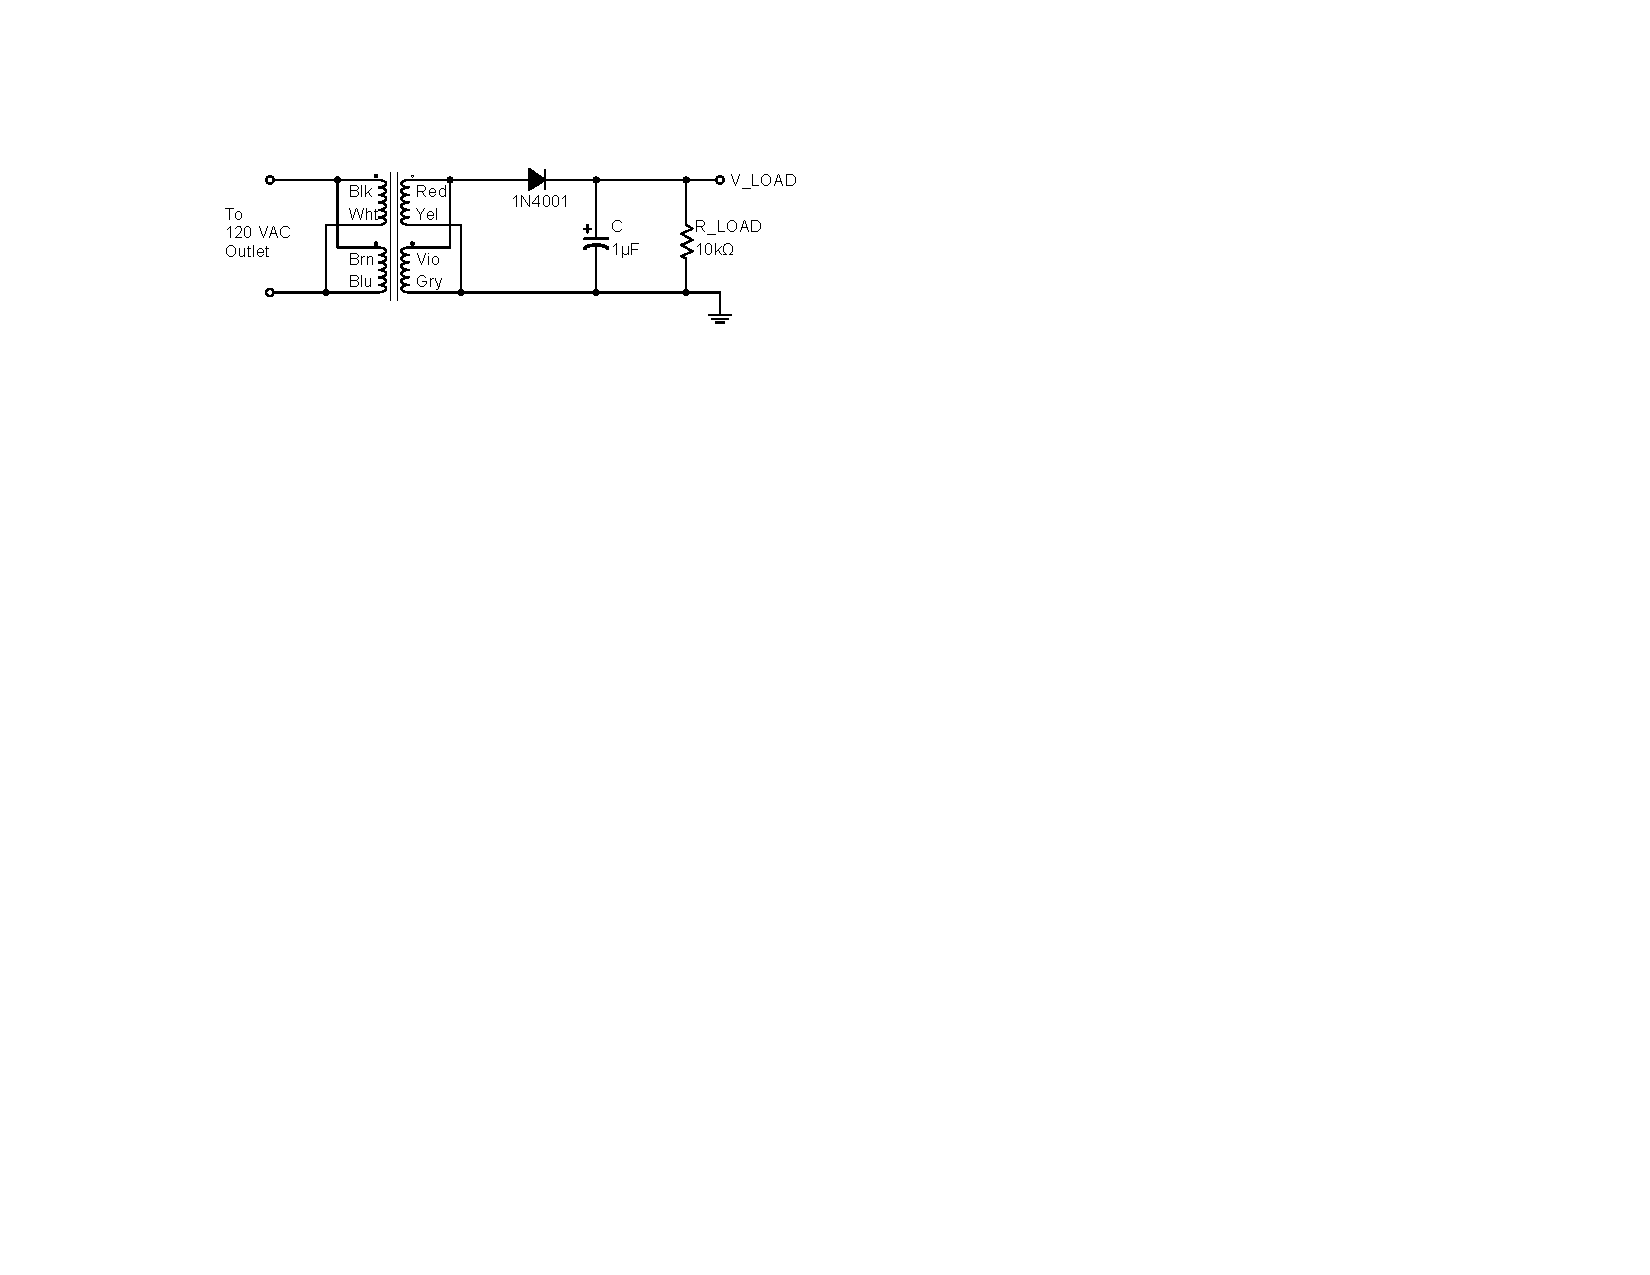
\includegraphics{power_supply/half_wave_rectifier.pdf}
\end{center}

\item Predict qualitatively what will happen to the minimum and maximum voltages across $R_{\rm load}$ if you double the value of $C$.  Test your prediction with a quantitative measurement.  

\item Predict qualitatively what will happen to the minimum and maximum voltages across $R_{\rm load}$ if you increase the load resistance to 100~k$\Omega$.  Test your prediction with a quantitative measurement. \label{part_ripple_measured}

\item The difference between the minimum and maximum voltages across $R_{\rm load}$ is called the ``ripple voltage'' $V_{\rm ripple}$, and generally you'd like it to be small.  In this part, you'll step through how to calculate the expected size of $V_{\rm ripple}$.  Suppose $C = 2~\mu$F, and $R_{\rm load}= 100$~k$\Omega$. \label{part_ripple_defined}

\begin{itemize}
\item Based on the maximum voltage you measured in part \ref{part_ripple_measured}, what is the maximum charge $Q$ on the capacitor?  What is the maximum current $I$ through the load?  \label{part_numerical_derivation}

\item How much charge $\Delta Q$ flows through the load in one cycle, assuming the current $I$ through the load is approximately constant for the whole cycle?  

\item By how much will that change $\Delta Q$ lower the voltage across the capacitor?  

\item Does your calculation match with the measurement you made part \ref{part_ripple_measured}?  
\end{itemize}

\item Follow the same steps as in part \ref{part_numerical_derivation} to calculate a general result for $V_{\rm ripple}$ in terms of $R_{\rm load}$, $C$,  $V_{\rm max}$, and the frequency $f$. \label{part_symbolic_derivation}

\item Calculate the size of capacitor required to lower the ripple voltage to 100~mV for a load of 100~k$\Omega$.  Test your calculation.  (As we continue to decrease the ripple voltage, you may find it handy to use the average function on your scope, under the acquire menu, to improve your measurements.)

\item Replace the half-wave rectifier with a full-wave bridge rectifier, shown below, using the 1N4001 for all the diodes.  As before, sketch the waveform of $V_{\rm load}$ both with and without the capacitor. \label{part_full_wave_bridge_rectifier}
\begin{center}
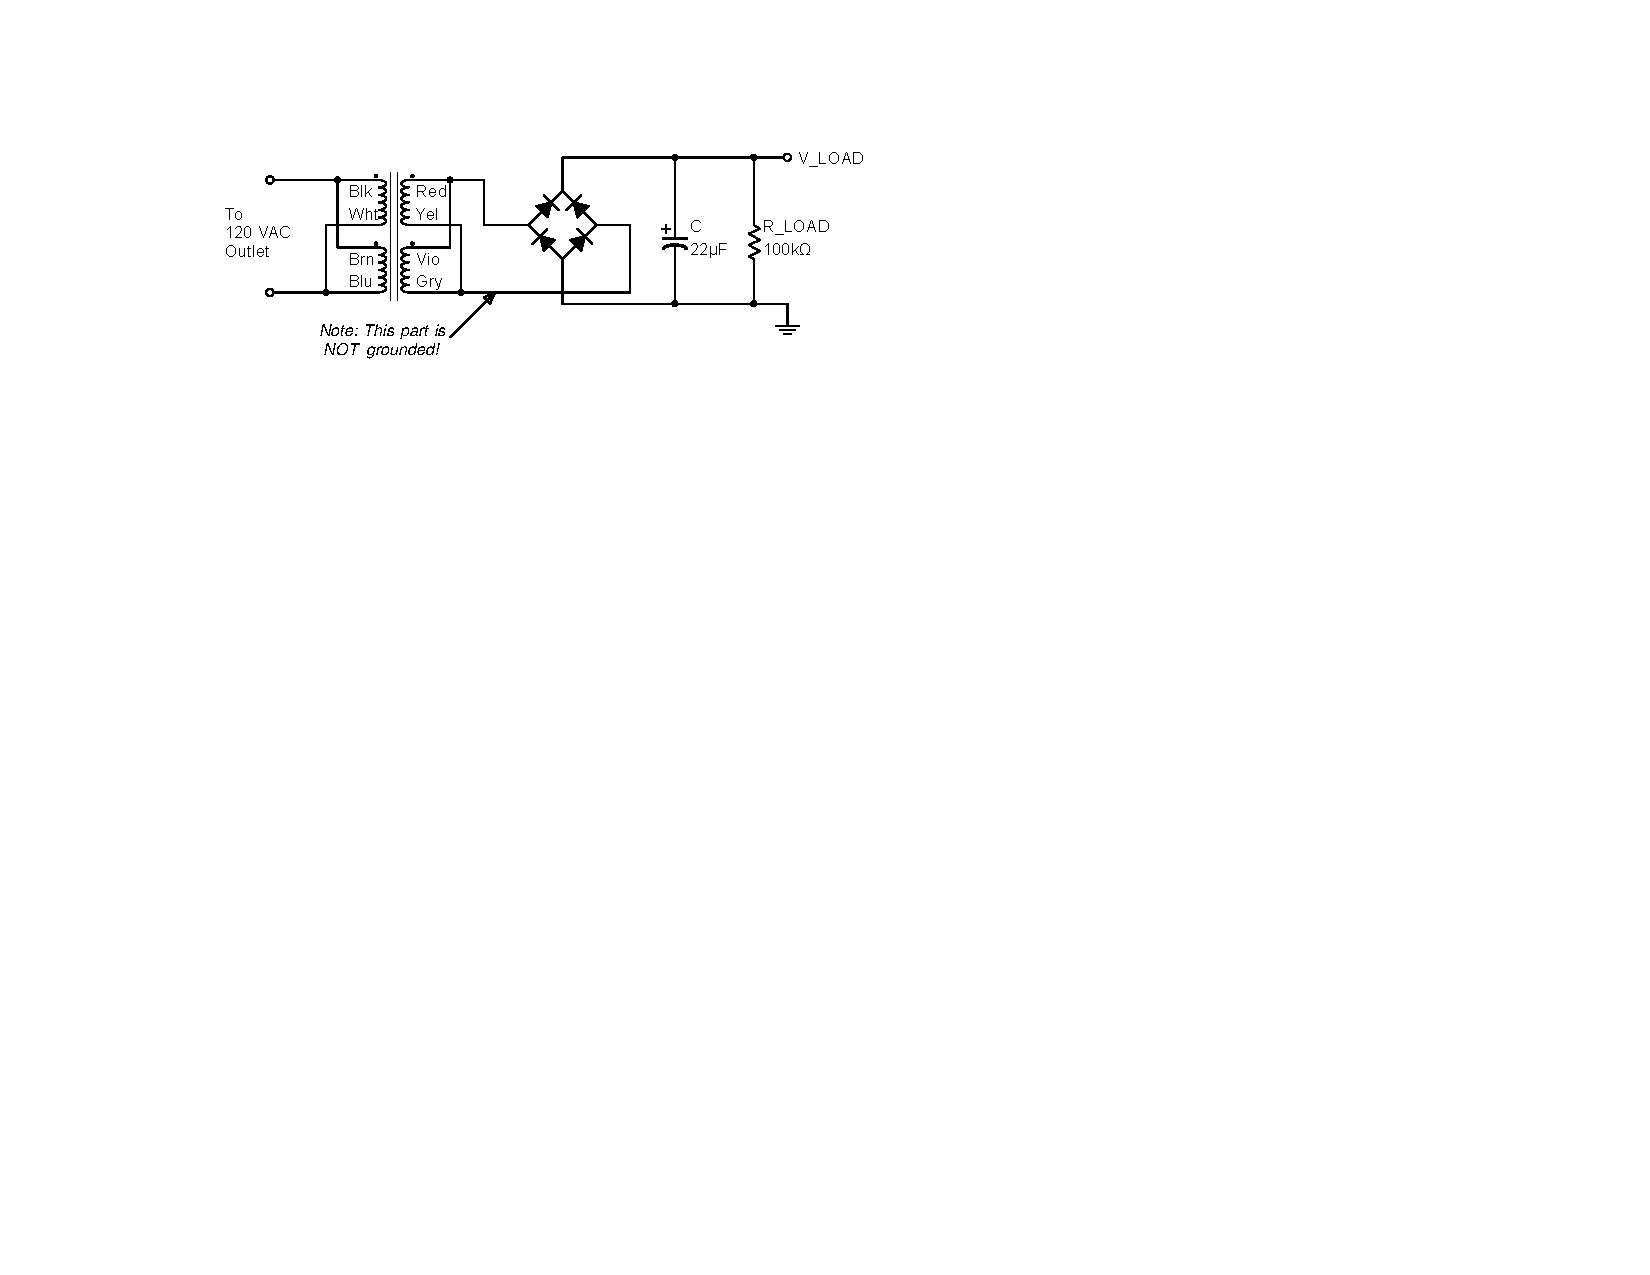
\includegraphics{power_supply/full_wave_bridge_rectifier.pdf}
\end{center}

\item With the capacitor in place, you can measure that the maximum voltage across $R_{\rm load}$ is slightly less than with the half wave rectifier.  How much less?  And why is that?

\item You should also see that the ripple voltage is about half what it was before.  Why is that?  Which part of your calculation in part \ref{part_symbolic_derivation} has effectively changed by a factor of two?  Rewrite your expression for $V_{\rm ripple}$ from part \ref{part_symbolic_derivation}, showing this tiny change needed for a full wave rectifier.  \label{part_symbolic_derivation_2f}

\item Replace the four diodes with the integrated bridge rectifier from your kits, and confirm that it works as predicted.  How are the leads labeled to indicate AC input and DC output?

\item To cut down the ripple voltage, you could of course make the capacitor much bigger, but that gets too large and too expensive pretty quickly.  A better way is to use a Zener shunt clipper, as shown below.  (The 1N4739 shown has a reverse breakdown voltage of $V_R=9$ volts.)  What value resistor is required for $R_{\rm lim}$ if we want to protect the diode by limiting the reverse current in the diode to about 4~mA?  (You should calculate that it's around 1~k$\Omega$.) Build the circuit and measure $V_{\rm ripple}$ and $V_{\rm DC}$ across the load, as well as the maximum and minimum of the voltage $V_C$ across the capacitor.  \label{part_zener_regulator}
\begin{center}
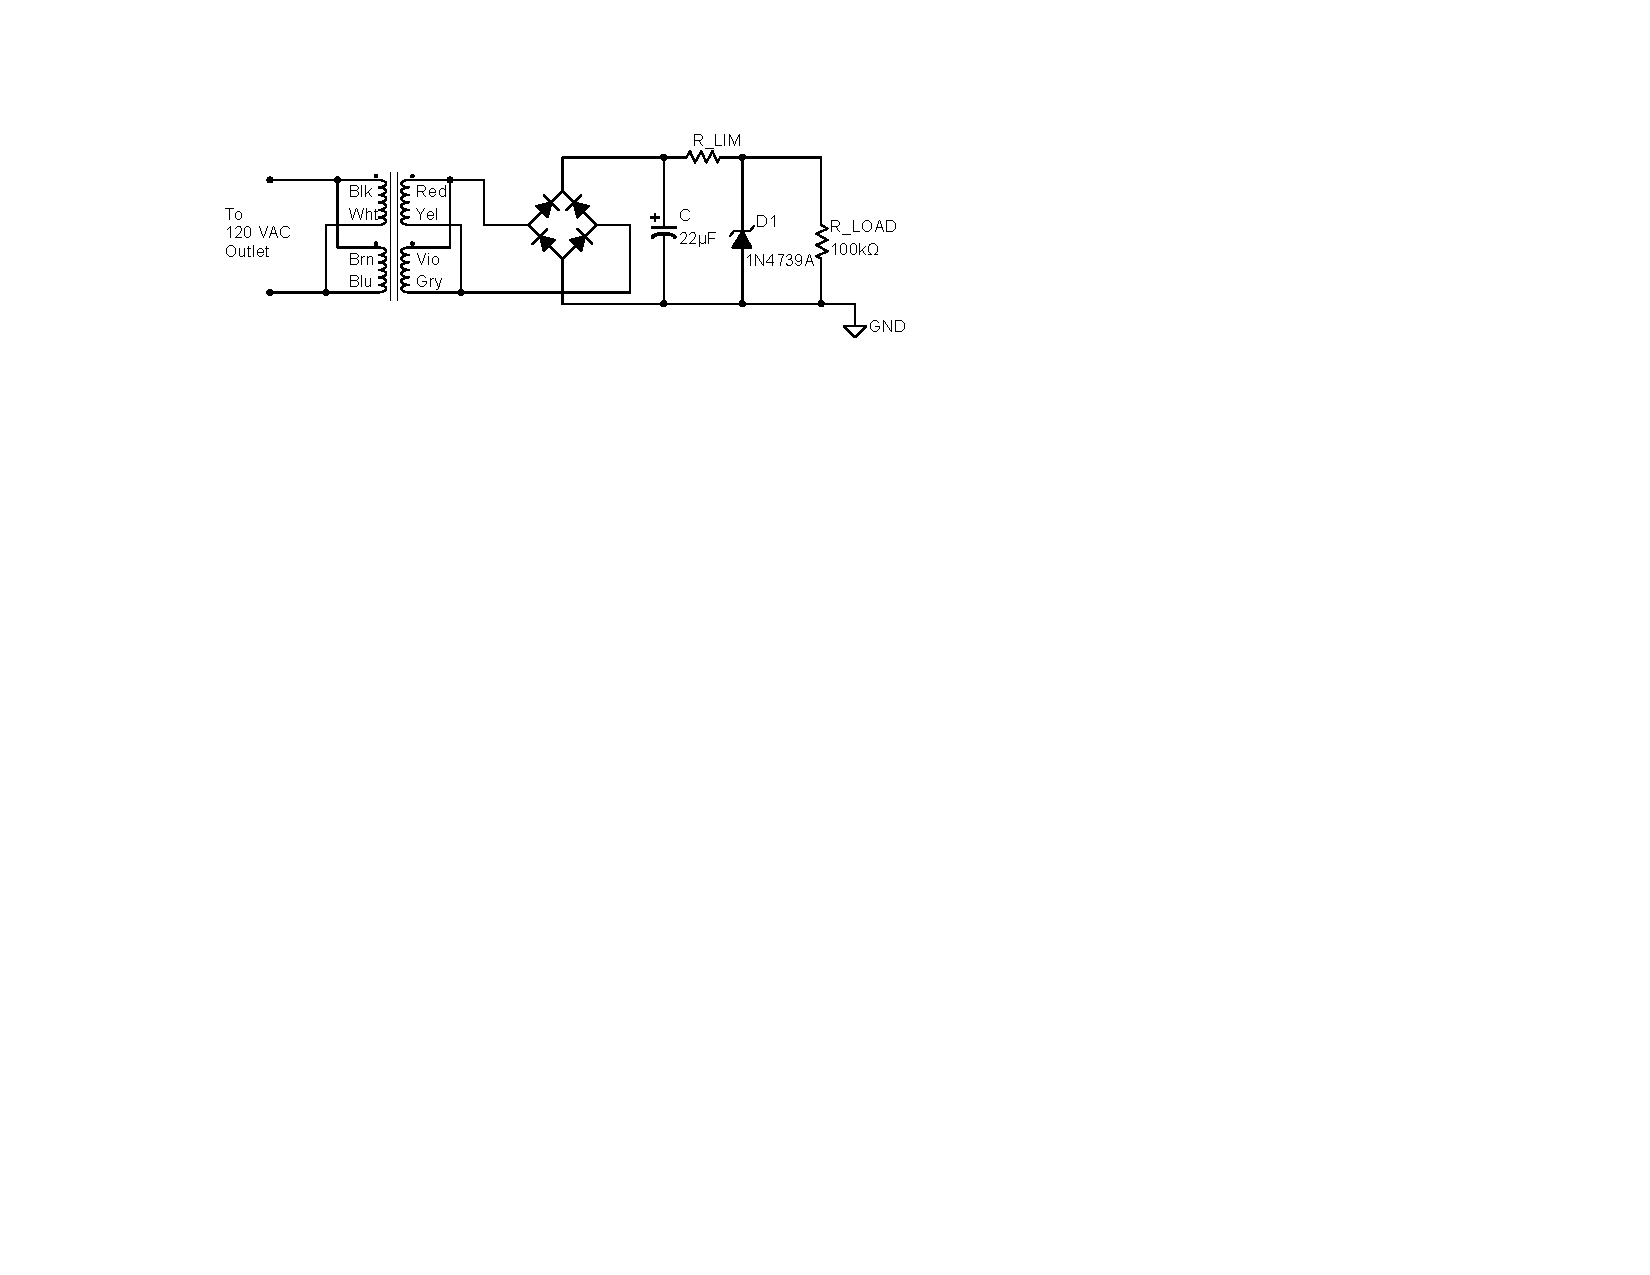
\includegraphics{power_supply/zener_regulator.pdf}
\end{center}

\item The circuit you just built should work fine as long as the value of $R_{\rm load}$ isn't too small.  But now what happens to your output when you change the load to $R_{\rm load} = 2.2$~k$\Omega$?  Why is your output no longer a steady 9 volts?

\item You can still make your circuit work with $R_{\rm load} = 2.2$~k$\Omega$ if you lower the value of $R_{\rm lim}$.  What is the largest value of $R_{\rm lim}$ that will make your circuit work?  (To make this problem doable, you can assume that you know that the ripple voltage at the capacitors will be about 2~volts.)  Fix your circuit using an ``extra safe'' value of $R_{\rm lim}=330$~$\Omega$ and redo the measurements you took in part~\ref{part_zener_regulator}.  \label{part_small_rlim}

\item Why is the output ripple voltage you found in part~\ref{part_small_rlim} larger than you found in part~\ref{part_zener_regulator}?  (Hint: draw a graph of the $IV$ curve for a Zener diode.  Are the vertical parts really exactly vertical?)

\item You have now seen the limitation of using a Zener shunt clipper for a DC power supply: for loads that draw large output currents, you need to lower $R_{\rm lim}$ so that the output voltage never falls below $V_R$ of the diode.  But small values of $R_{\rm lim}$ draw more current, which leads to larger ripple voltages, and would eventually lead to currents that would damage the diode.  And fundamentally, the output ripple voltage is \textit{always} going to be a problem for large currents, because the voltage across the diode isn't exactly 9.00000 volts---it always depends a little on the current in the diode.  So you can't win!  Fortunately, there's a terrific solution to all of these problems, and it comes in a little chip that costs just pennies and can happily output 100 mA.  Build the circuit shown below, and verify that it produces a smooth 9 V output. \label{part_linear_power_supply_78xx}
\begin{center}
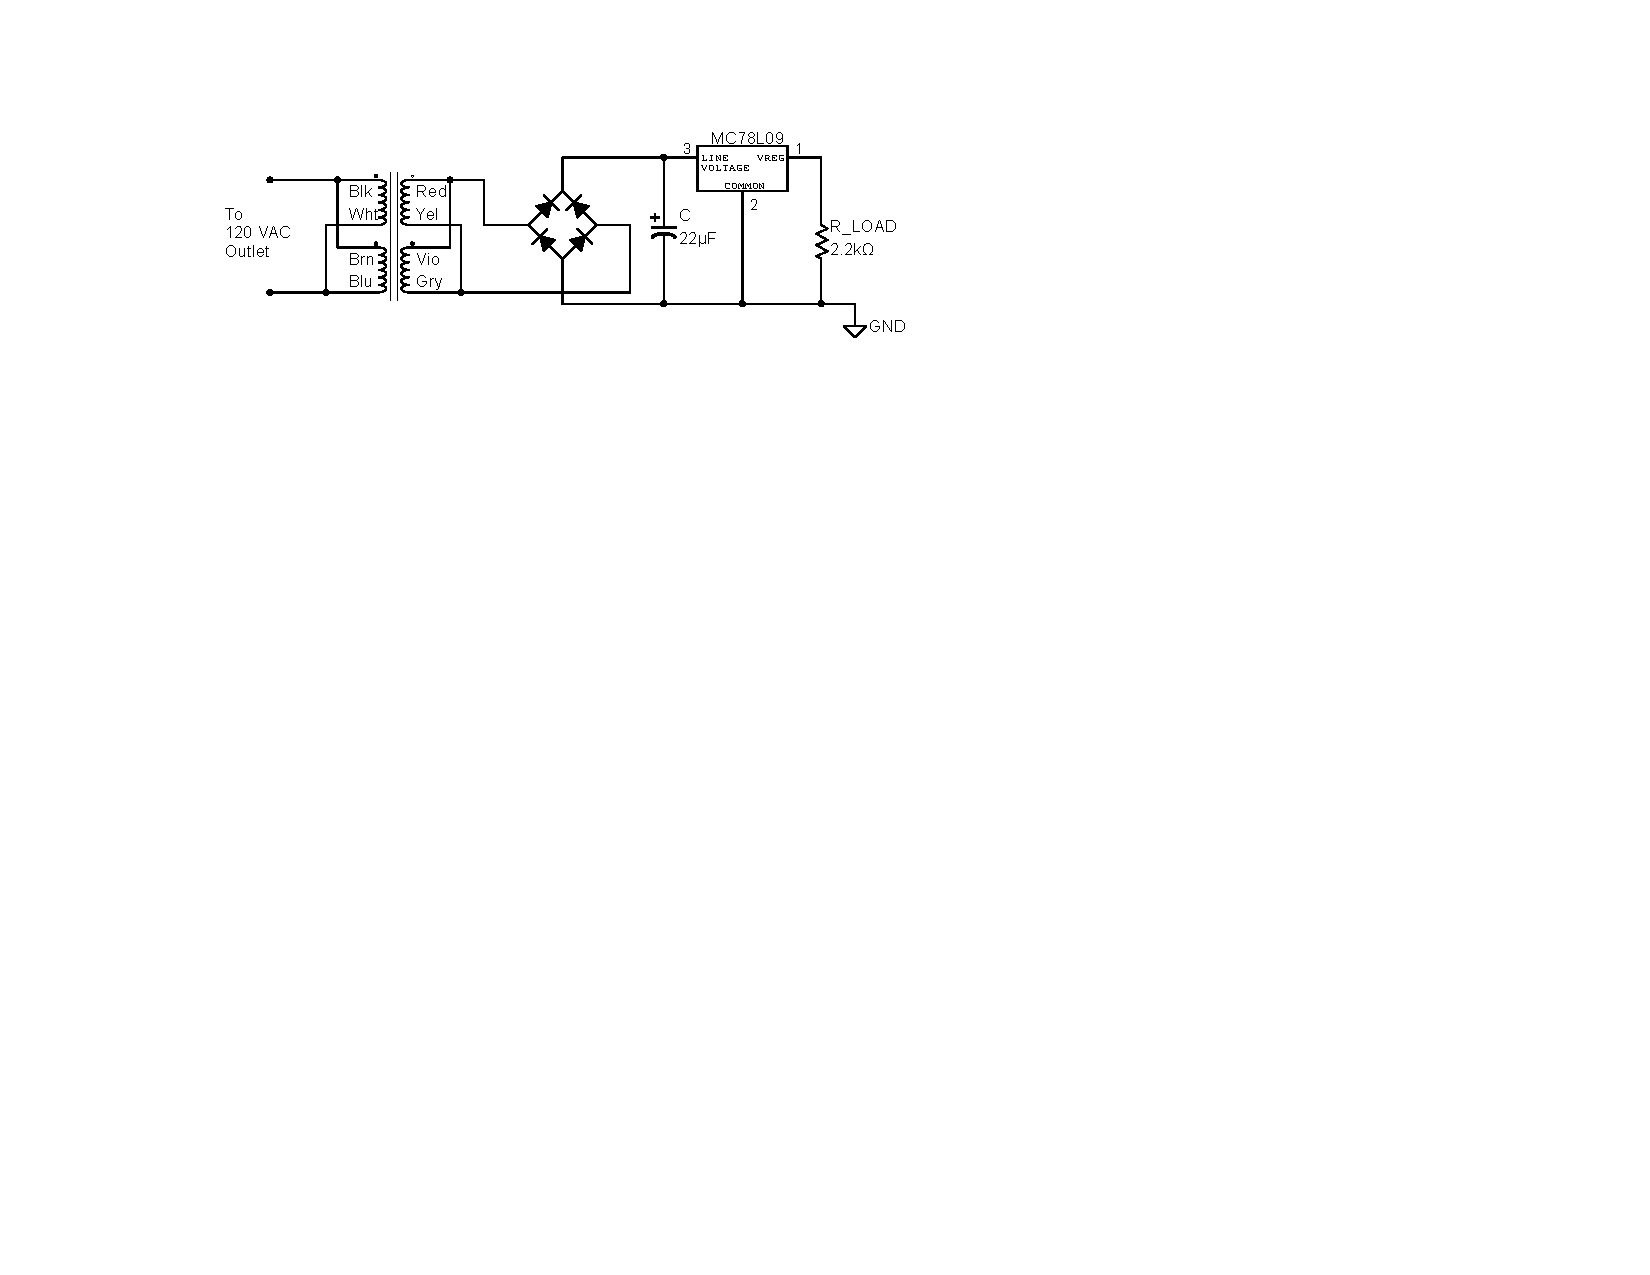
\includegraphics{power_supply/7809_regulator.pdf}
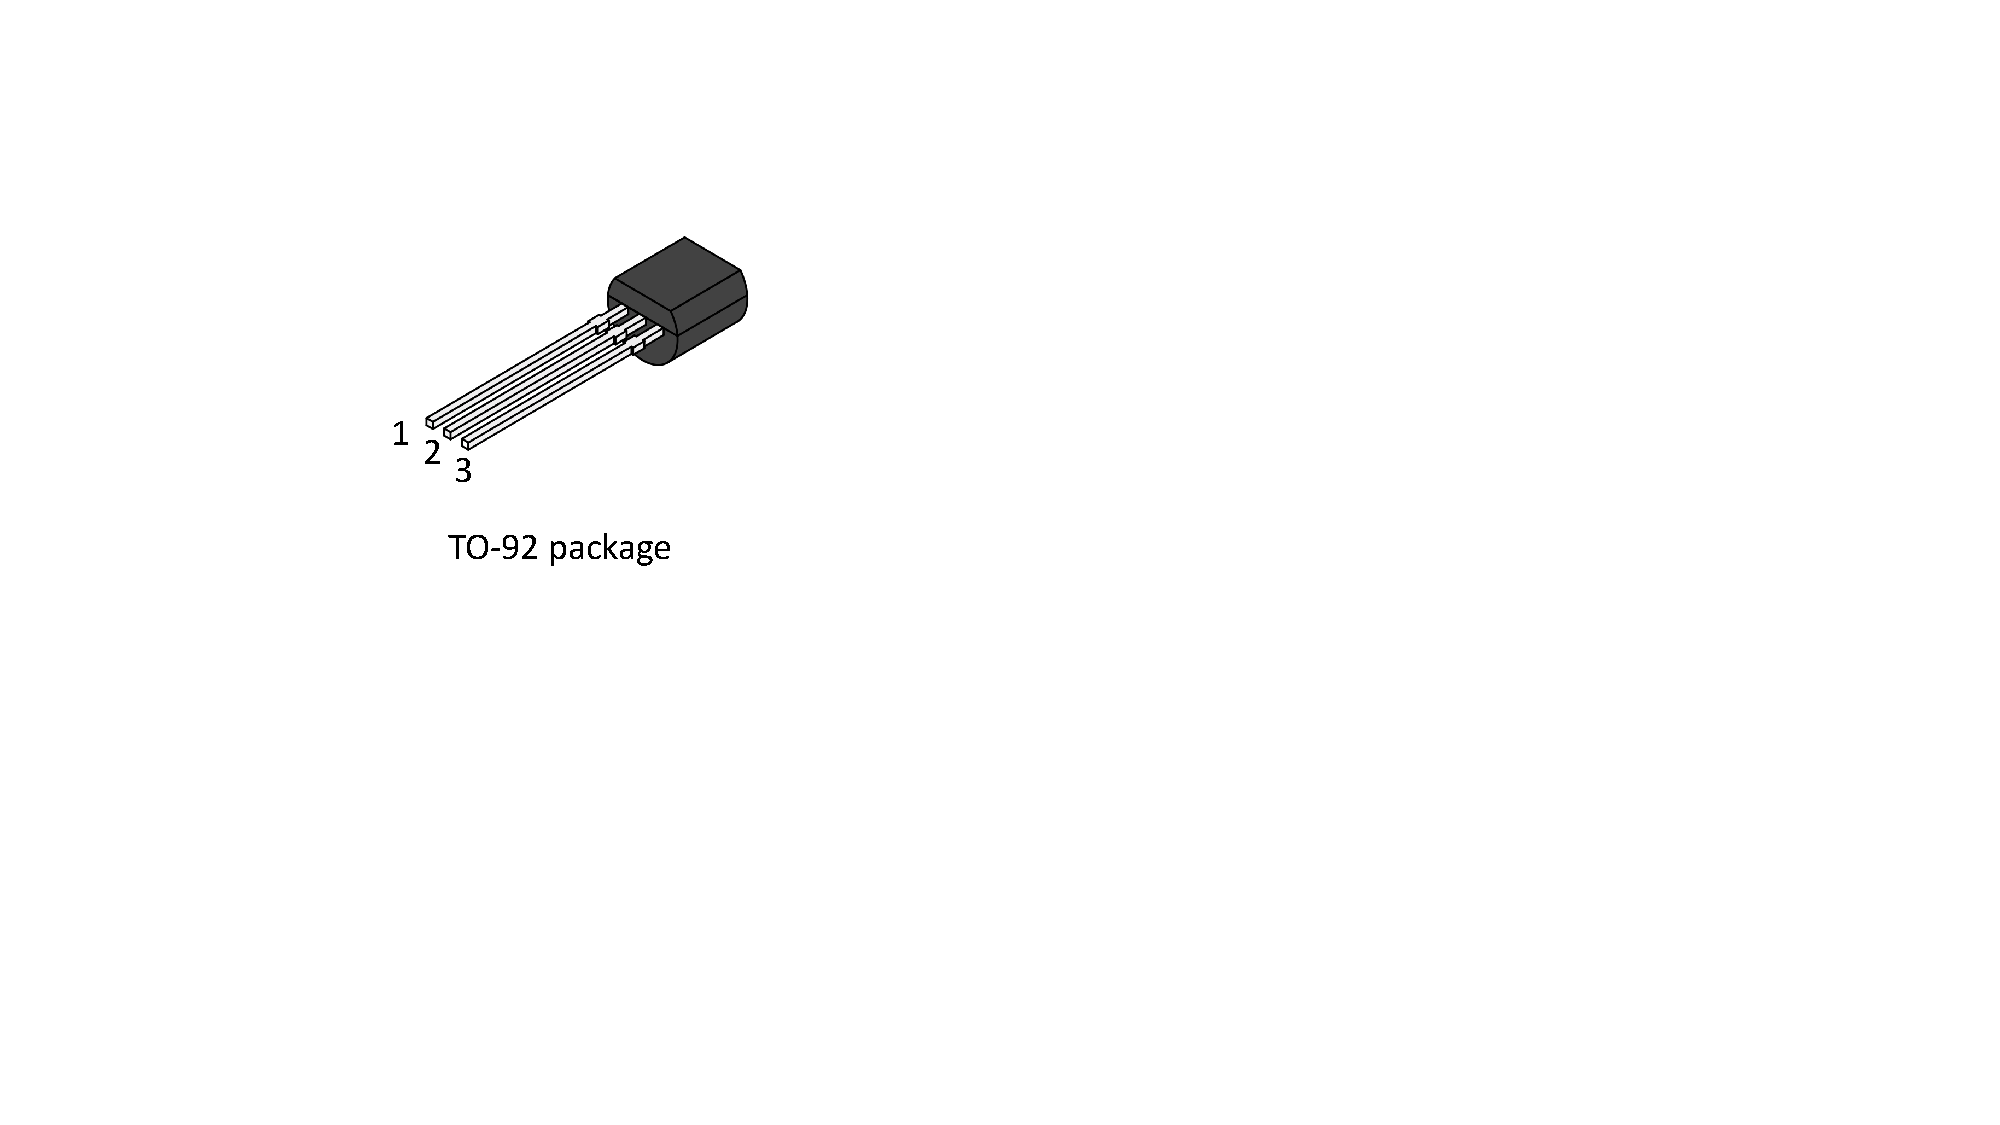
\includegraphics[width=1.3in]{appendices/pinouts/TO-92_package_pinout.pdf}
\end{center}
 
\item Using the two channels of your oscilloscope to simultaneously measure the input and output voltages of the MC78L09, what happens to those voltages when you change the capacitor to $C = 10$~$\mu$F?  Why this huge change in the output?  (Hint: Look up the ``dropout voltage'' on its data sheet.  Be sure you're using the data sheet for the small MC78L09, in the TO-92 package.)

\item Because of the dropout voltage of your MC78L09, you need to maintain an input voltage of at least 10.7 volts for the regulator to function properly.  With that in mind, what capacitance $C$ would you need to use if your load resistance were small enough to draw 100~mA?   (Hint: Rewrite your expression for ripple voltage from part~\ref{part_symbolic_derivation_2f} in terms of the load current.)

\item Using $R_{\rm load} = 2.2$~k$\Omega$ and $C = 22$~$\mu$F, measure the ripple voltage across $R_{\rm load}$, and compare that to the ripple voltage at the input of the MC78L09.  By what factor has this ripple voltage been reduced?  How does that compare to the value stated on the data sheet, which is given in dB?

\item You also have in your kits an MC7805, in a larger TO-220 package.  How much output current are these capable of?  What is their ``ripple rejection'' ratio, in dB?  How big would $V_{\rm ripple}$ be if you used this in your circuit above?  (No need to build this one.)

\end{enumerate}

\textbf{Possible Exam Questions:}

\begin{itemize}
%\item Use a transformer, four silicon diodes, one capacitor, and a 7805 regulator to design a power supply to design a power supply that delivers 5 volts at 300~mA with 0.1~mV ripple.  The 7805 has ripple rejection of 75~dB and a dropout voltage of 1.7 volts.  Specify the capacitance and transformer turns ratio required.

\item Derive the expression $V_{\rm ripple}=V_{\rm max}/2fR_{\rm load} C$.

\item Draw a circuit diagram showing how to use a Zener shunt clipper as a voltage regulator.  Do these work best at high currents or low currents?  What two problems will you face if you push these past their useful current range?

\item Draw a half wave rectifier and a full wave rectifier.  Which requires a larger capacitor to yield the same ripple voltage?  Which has a slightly larger voltage drop across it, thus dissipating slightly more power and lowering its efficiency?

\item What does the ``dropout voltage'' of a voltage regulator mean?  What does the ``ripple rejection'' ratio of a regulator mean?  What are typical values of these quantities? 

\end{itemize}






